\chapter{Adaptive Query Execution}
\label{ch:aqe}

\begin{chapterintro}
The specimen's join stage shuffles into 200 partitions, a number the planner
chose before it had seen a single byte. In the week of the viral product, one
of those partitions holds 3.2~GB while the median holds 40~MB, and the stage
finishes only when the task reading that one partition does. Raise
\conf{spark.sql.shuffle.partitions} to 2000 for the other stages and the
opposite problem appears: thousands of tasks, each moving a few megabytes.
Adaptive Query Execution (AQE) fixes both by measuring after each shuffle and
re-planning what has not yet run. This chapter covers what AQE re-decides, from
what evidence, how to read the plan that results, and the places where it
cannot help.
\end{chapterintro}

\section{Why runtime beats planning time}
\label{sec:aqe-why}

Every decision in \Cref{ch:catalyst} and \Cref{ch:joins} --- how many shuffle
partitions, which join strategy, whether to broadcast --- is made from an
\emph{estimate}: a file size, a row count, a number the catalog may or may not
have. The estimate is wrong in predictable ways. A filter's selectivity is
guessed, a join's output cardinality is guessed from guesses, and a Parquet
file's on-disk size says little about its decoded size
(\Cref{sec:mem-heap}). The optimizer cannot do better, because the data has
not moved yet.

\emph{Adaptive Query Execution} is Spark inserting a measurement after every
shuffle. Once a shuffle has run, Spark knows the exact byte size of every
partition it produced --- no estimation error, no missing statistics. AQE uses
that certainty to re-plan the stages that have not run. It has been on by
default since Spark 3.2 (\conf{spark.sql.adaptive.enabled}), and there is
little reason to turn it off.

\begin{analogy}
Planning without AQE is plotting a road trip from a map: you pick the route
once, before leaving, from the distances printed on it. AQE adds a checkpoint
at every toll booth where you read the real traffic and may take a different
exit. The analogy breaks in one place that matters: you can change only the road
\emph{after} the toll booth. The miles already driven, and the booths you
decided to pass through, stay as they were.
\end{analogy}

That limit is the chapter's second theme. AQE cannot change a stage that has
already run, and it cannot remove a shuffle that planning decided was necessary.
It optimizes what happens after the measurement, not before it. The rest of the
chapter walks the three things it does re-decide, then the limits.

\section{The feedback loop}
\label{sec:aqe-loop}

\Cref{fig:aqe-feedback-loop} shows the mechanism that all three optimizations
share. Without AQE, Spark turns the physical plan into stages once, at the start,
and runs them in order. With AQE, the driver cuts the plan at every
\texttt{Exchange} into \emph{query stages}: a query stage is a piece of the plan
that is materialized (run to completion, its output written as shuffle files or
collected for a broadcast) before anything downstream of it is planned in
detail. The wrapper node that owns this loop is \texttt{AdaptiveSparkPlan}.

\begin{figure}[htbp]
  \centering
  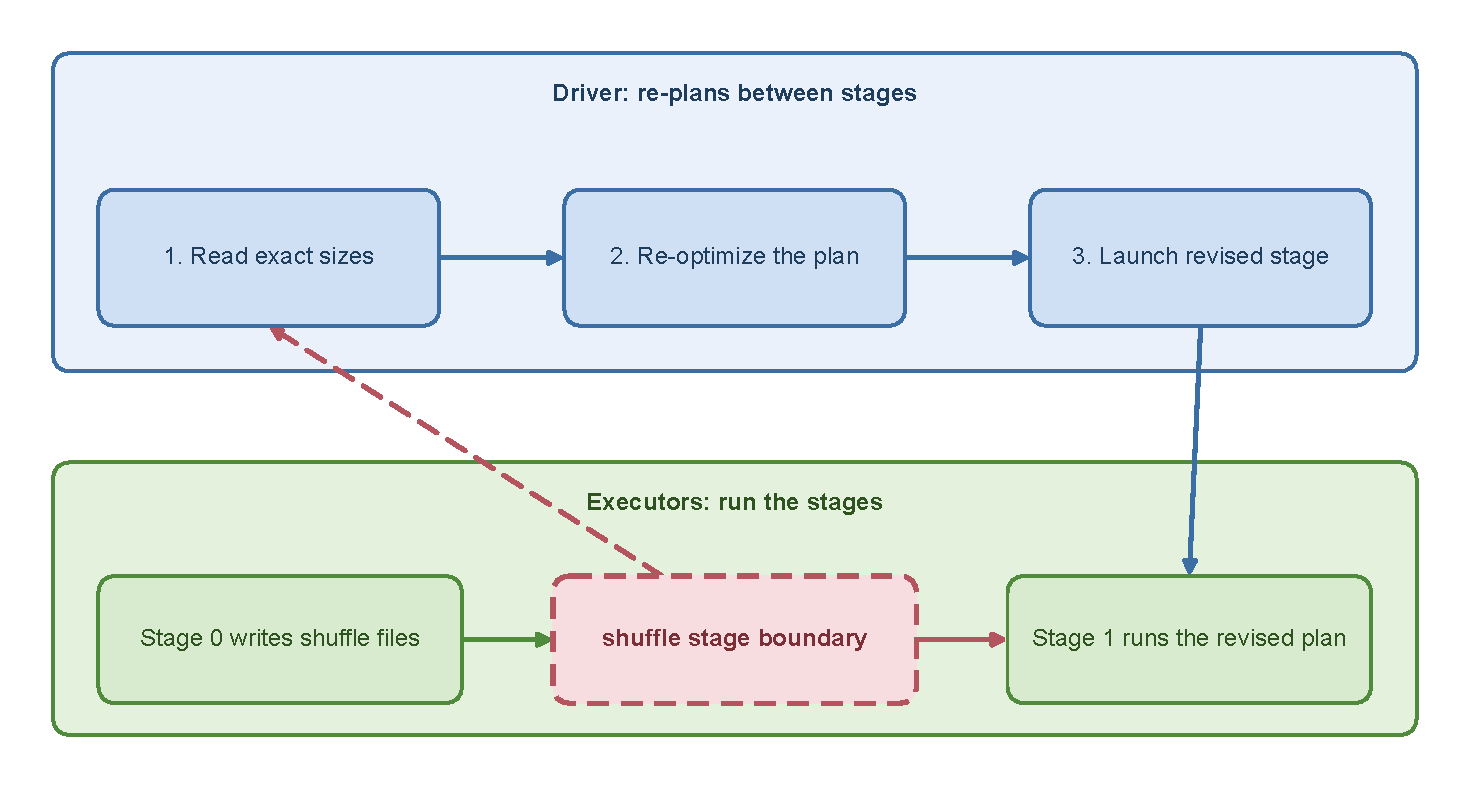
\includegraphics[width=\linewidth]{aqe-feedback-loop.pdf}
  \caption{AQE inserts a measurement between stages: when a shuffle finishes,
  the driver reads the exact size of every output partition and re-optimizes
  only the part of the plan that has not run. Blue steps run on the driver,
  green on the executors; the rose dashed box is the stage boundary where the
  measurement happens.}
  \label{fig:aqe-feedback-loop}
\end{figure}

The loop has three steps. First, a query stage finishes and reports its
\emph{map output statistics}: the exact byte size of every shuffle partition.
Second, the driver substitutes those measured sizes for the estimates in the
logical plan that remains, and runs the optimizer again over only that
unfinished part. Third, it plans the physical operators for the next query stage
from the result and launches it. Then the loop repeats, once per shuffle, until
no exchange remains.

Three rewrites fall out of this one loop, and the rest of the chapter takes them
in turn. \Cref{tab:aqe-rewrites} names each next to its planning-time
counterpart, so you can see that AQE does not add new kinds of decision; it
revisits decisions Catalyst already made and gives them evidence.

\begin{table}[htbp]
\centering\footnotesize
\renewcommand{\arraystretch}{1.25}
\begin{tabular}{@{}p{2.7cm}p{3.5cm}p{3.5cm}p{4.0cm}@{}}
\toprule
\textbf{AQE rewrite} & \textbf{Planning-time decision it revisits} & \textbf{Evidence it uses} & \textbf{Where it shows up in the plan} \\
\midrule
Coalesce partitions & shuffle partition count (\Cref{sec:shuffle-sizing}) & byte size of every partition & \texttt{AQEShuffleRead coalesced} \\
Broadcast promotion & join strategy (\Cref{sec:joins-selection}) & total bytes of one shuffled side & \texttt{BroadcastHashJoin}, \texttt{BroadcastQueryStage} \\
Skew split & one partition per key range & partition size against the median & \texttt{AQEShuffleRead skewed}, \texttt{isSkew=true} \\
\bottomrule
\end{tabular}
\caption{The three runtime rewrites, each a planning-time decision revisited
with measured evidence.}
\label{tab:aqe-rewrites}
\end{table}

Before running the specimen, ask for its plan:

\begin{lstlisting}[language=SQL,caption={Asking for the plan before the query runs},captionpos=b,label=lst:aqe-explain-before]
EXPLAIN FORMATTED
SELECT p.category,
       AVG(CASE WHEN o.delivery_days <= o.promised_days THEN 1.0 ELSE 0.0 END) AS on_time_rate
FROM orders o
JOIN dim_product p ON o.product_id = p.product_id
WHERE o.order_ts >= TIMESTAMP '2026-03-01 00:00:00'
  AND o.order_ts <  TIMESTAMP '2026-03-08 00:00:00'
GROUP BY p.category;
\end{lstlisting}

The root of what comes back is \texttt{AdaptiveSparkPlan isFinalPlan=false}. That
flag is the point: this is the plan Spark \emph{intends} to run, and it may
change at every query stage boundary. The plan that actually ran is a different
object, and \Cref{sec:aqe-reading} shows how to read it. % CAPTURE: EXPLAIN FORMATTED of lst:aqe-explain-before on the reference cluster

\section{Coalescing shuffle partitions}
\label{sec:aqe-coalesce}

\Cref{sec:shuffle-sizing} recommended setting
\conf{spark.sql.shuffle.partitions} generously and letting AQE bring the count
back down. This is the mechanism that does it. After a shuffle, AQE reads the
exact size of every partition and merges \emph{adjacent} ones until each is close
to a target size (\Cref{fig:aqe-coalesce}). The count you set is only a ceiling:
Spark starts from \conf{spark.sql.shuffle.partitions} partitions, or from
\conf{spark.sql.adaptive.coalescePartitions.initialPartitionNum} if you set that
instead, and merges down from there.

\begin{figure}[htbp]
  \centering
  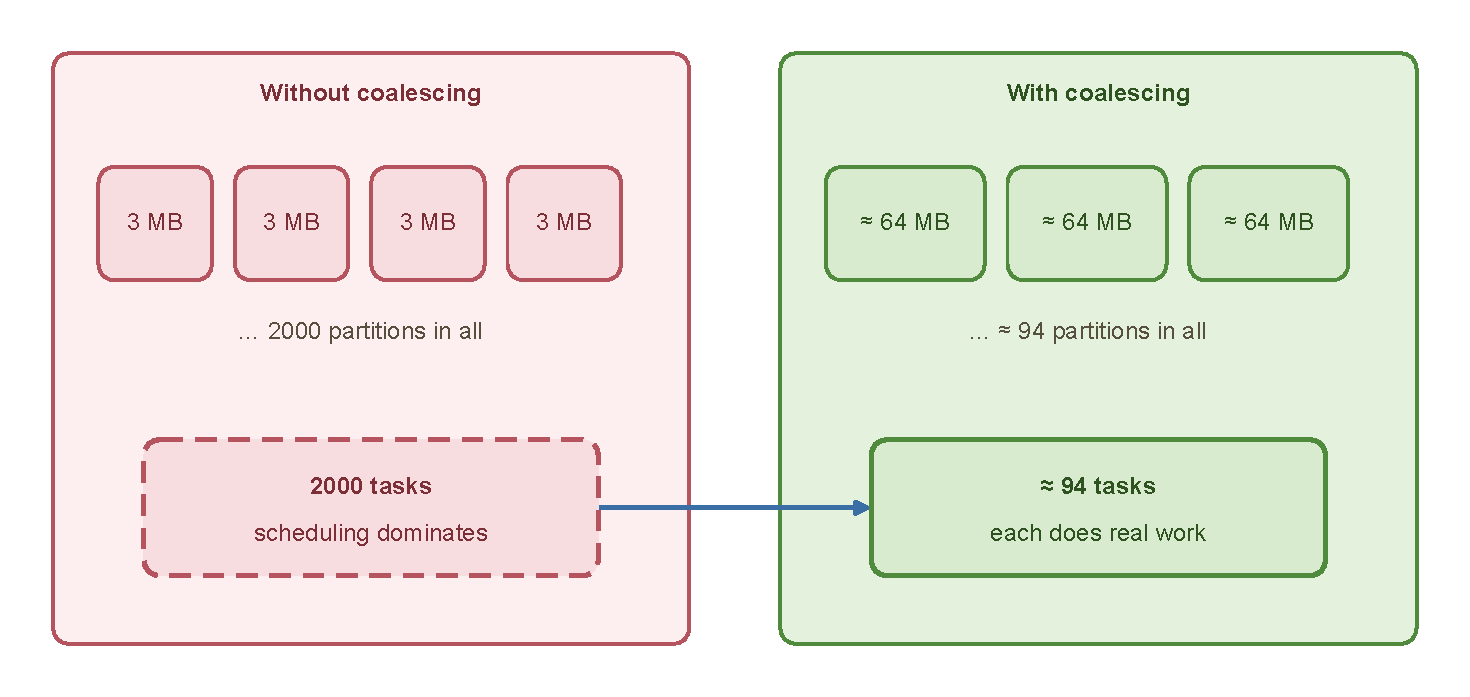
\includegraphics[width=\linewidth]{aqe-coalesce.pdf}
  \caption{2000 shuffle partitions of 3~MB each carry 6~GB; AQE merges adjacent
  partitions toward the 64~MB advisory size, so the next stage runs about 94
  tasks instead of 2000. Rose marks the cost, green the corrected state.}
  \label{fig:aqe-coalesce}
\end{figure}

\subsection{The target size, and what parallelism does to it}
\label{sec:aqe-parallelism}

The target is where most readers go wrong, because two keys influence it.
\conf{spark.sql.adaptive.advisoryPartitionSizeInBytes} defaults to 64~MB. \conf{spark.sql.adaptive.coalescePartitions.minPartitionSize} (1~MB)
is a floor that stops AQE from producing absurdly small partitions. And
\conf{spark.sql.adaptive.coalescePartitions.parallelismFirst} (default
\texttt{true}) tells Spark not to merge so far that the cluster goes idle.
With \texttt{parallelismFirst} on, the effective target is

\[
\text{target} \;=\; \max\!\Bigl(\min\!\bigl(\tfrac{\text{total shuffle bytes}}{P},\ \text{advisory size}\bigr),\ \text{min partition size}\Bigr),
\]

where $P$ is the cluster's default parallelism, which on the reference cluster
is its 40 task slots (\Cref{app:refenv}). In words: the advisory size is a
\emph{ceiling} on the target, and the parallelism term pulls it lower whenever
the shuffle is small enough that 64~MB partitions would leave slots idle. Turn
\texttt{parallelismFirst} off and the formula collapses to the advisory size
alone. (Claim --- verify against \texttt{ShufflePartitionsUtil} in the 3.5 source
and with the capture in \Cref{lst:aqe-coalesce-plan}; the Spark docs describe
the setting as ignoring the advisory size, which is true in the small-shuffle
case below but not in the large one.)

\Cref{tab:aqe-parallelism-first} puts numbers on it for the reference cluster.

\begin{table}[htbp]
\centering\footnotesize
\renewcommand{\arraystretch}{1.25}
\begin{tabular}{@{}rrrrrr@{}}
\toprule
\textbf{Shuffle} & $P$ & \textbf{Target (\texttt{true})} & \textbf{Parts.} & \textbf{Target (\texttt{false})} & \textbf{Parts.} \\
\midrule
6~GB    & 40 & $\min(150, 64)$ = 64~MB & $\approx$ 94 & 64~MB & $\approx$ 94 \\
1.5~GB  & 40 & $\min(37.5, 64)$ = 37.5~MB & 40 & 64~MB & $\approx$ 24 \\
200~MB  & 40 & $\min(5, 64)$ = 5~MB & 40 & 64~MB & $\approx$ 4 \\
20~MB   & 40 & $\max(\min(0.5, 64), 1)$ = 1~MB & $\approx$ 20 & 64~MB & 1 \\
\bottomrule
\end{tabular}
\caption{Coalescing a shuffle on 40 slots, with \texttt{parallelismFirst} true
and false. Partition counts are approximate:
AQE merges greedily in partition order, so real counts differ slightly. With
\texttt{parallelismFirst} on, a small shuffle keeps as many partitions as there
are slots; with it off, the same shuffle collapses to a handful of tasks and
leaves most of the cluster idle.}
\label{tab:aqe-parallelism-first}
\end{table}

The first row is the case \Cref{fig:aqe-coalesce} draws: 6~GB divided over 40
slots is 150~MB per slot, far above the 64~MB advisory size, so the advisory
size wins and the stage runs about $6000 / 64 \approx 94$ tasks, two to three
waves over 40 slots. The second and third rows are where \texttt{parallelismFirst}
earns its default: 1.5~GB at 64~MB would give 24 tasks on 40 slots, one wave with
16 cores idle, while the parallelism term keeps all 40 busy. The fourth row shows
the floor: with only 20~MB to move, nothing smaller than 1~MB is worth a task.

\begin{warning}
$P$ is Spark's \emph{default parallelism}, which is the number of cores the
application holds \emph{right now} unless you set
\conf{spark.default.parallelism}. Under dynamic allocation
(\Cref{ch:tuning}) a query that starts while the application holds few
executors sees a small $P$, and AQE coalesces harder than the cluster you
eventually get could use. (Claim --- verify on your cluster by comparing the
partition count in \Cref{lst:aqe-coalesce-plan} across a cold and a warm
application.)
\end{warning}

When you want AQE to respect the advisory size exactly --- say, you are sizing
partitions for a downstream write and the 40-slot term only gets in the way ---
set \texttt{parallelismFirst} to \texttt{false}:

\begin{lstlisting}[language=SQL,caption={Making the advisory size binding},captionpos=b,label=lst:aqe-coalesce-settings]
SET spark.sql.adaptive.coalescePartitions.parallelismFirst=false;
SET spark.sql.adaptive.advisoryPartitionSizeInBytes=134217728;  -- 128 MB
\end{lstlisting}

\Cref{sec:shuffle-sizing}'s recommended settings use exactly this pairing; the
first line is what makes the second one do what the second line says.

\subsection{Seeing it in the plan}

When coalescing fires, the final plan carries an \texttt{AQEShuffleRead} node
marked \texttt{coalesced} over the shuffle's query stage:

\begin{lstlisting}[language=text,numbers=none,caption={The shape of a coalesced shuffle read in a final plan},captionpos=b,label=lst:aqe-coalesce-plan]
AdaptiveSparkPlan isFinalPlan=true
+- HashAggregate(keys=[category], functions=[avg(...)])
   +- AQEShuffleRead coalesced
      +- ShuffleQueryStage 1
         +- Exchange hashpartitioning(category, 2000)
            +- HashAggregate(keys=[category], functions=[partial_avg(...)])
               +- ... scan, filter, join ...
\end{lstlisting}
% CAPTURE: final plan of the specimen on the reference cluster; record the post-coalesce partition count from the AQEShuffleRead node's "number of partitions" metric in the SQL tab

The \texttt{Exchange} still says 2000, because that is what was planned and what
the map side wrote. The coalescing is a property of the \emph{read}: the reduce
tasks fetch several adjacent map-side partitions as one. No data is rewritten.
That is why coalescing is free: the shuffle files are already on disk, and AQE
only changes how many reduce tasks read them.

\begin{tip}
Merging is one-directional. AQE only ever combines \emph{adjacent} small
partitions into fewer, larger ones; it never splits an oversized partition this
way. An oversized partition is handled by a different mechanism
(\Cref{sec:aqe-skew}), and coalescing does nothing for it.
\end{tip}

\section{Converting sort-merge to broadcast at runtime}
\label{sec:aqe-broadcast}

\Cref{sec:joins-selection} chooses a join strategy from an estimate, and the
estimate for the specimen's \texttt{dim\_product} was too high to broadcast. AQE
gets a second chance after that table's own shuffle. It adds up the bytes in
every shuffle partition on that side, and if the total is below the adaptive
threshold, it rewrites the sort-merge join into a broadcast hash join before the
join runs. The final plan shows \texttt{BroadcastHashJoin} where the plan had
\texttt{SortMergeJoin}, with a \texttt{BroadcastQueryStage} holding the small
side.

\subsection{What the conversion saves, and what it cannot}

The conversion arrives after both sides of the join have shuffled, because AQE
cannot measure a shuffle that has not run. That fixes what the rewrite is able
to save. The big side's map-side shuffle \emph{write} has already happened and is
not undone; the savings are the sort-merge join's costs that come after it: the
network fetch of the big side, and sorting both sides. To avoid the fetch, AQE
reads the big side with a \emph{local shuffle reader}
(\conf{spark.sql.adaptive.localShuffleReader.enabled}, default \texttt{true}):
each reduce task reads shuffle files from its own executor instead of pulling a
slice from every executor. The plan marks it \texttt{AQEShuffleRead local}.

\begin{lstlisting}[language=text,numbers=none,caption={The shape of a runtime broadcast promotion},captionpos=b,label=lst:aqe-broadcast-plan]
AdaptiveSparkPlan isFinalPlan=true
+- HashAggregate(keys=[category], functions=[avg(...)])
   +- ...
      +- BroadcastHashJoin [product_id], [product_id], Inner, BuildRight
         :- AQEShuffleRead local
         :  +- ShuffleQueryStage 0
         +- BroadcastQueryStage 2
            +- BroadcastExchange HashedRelationBroadcastMode(...)
               +- ShuffleQueryStage 1
\end{lstlisting}
% CAPTURE: final plan of the specimen under lst:aqe-promotion-experiment; check the exact BuildRight/BuildLeft and the local-reader annotation

Compare this to a join Catalyst broadcast at planning time. There, the big side
is never shuffled at all, and Spark saves the map-side write too. A runtime
promotion is the consolation prize, not the equal: you still pay the shuffle you
planned. When a side is reliably small, a hint or \texttt{ANALYZE}
(\Cref{sec:joins-forcing}) is still the better fix, because it prevents the
shuffle instead of salvaging half of it.

\subsection{The two broadcast thresholds}
\label{sec:aqe-thresholds}

\conf{spark.sql.autoBroadcastJoinThreshold} and
\conf{spark.sql.adaptive.autoBroadcastJoinThreshold} are two separate keys.
Confusing them is easy because the second has no default of its own: when unset,
it takes the value of the first, 10~MB. They compare against different
evidence, as \Cref{tab:aqe-thresholds} sets out.

\begin{table}[htbp]
\centering\footnotesize
\renewcommand{\arraystretch}{1.25}
\begin{tabular}{@{}p{3.3cm}p{5.5cm}p{5.5cm}@{}}
\toprule
 & \textbf{Planning-time threshold} & \textbf{Adaptive threshold} \\
\midrule
Key & \conf{spark.sql.autoBroadcastJoinThreshold} & \conf{spark.sql.adaptive.autoBroadcastJoinThreshold} \\
Default & 10~MB & unset, so the same as the planning key \\
Compared against & an estimate: catalog statistics, or file sizes & the measured total of the shuffle output on that side \\
What can go wrong & the estimate is low and the real table is large; the driver or executors run out of memory & the shuffle bytes understate the in-memory size, because shuffle data is compressed \\
Decided & before any stage runs & after the side's shuffle stage finishes \\
\bottomrule
\end{tabular}
\caption{The two thresholds guard against different failures. The planning-time
one must stay conservative because its input is a guess; the adaptive one sees
a real number, but a real number of \emph{compressed shuffle bytes}.}
\label{tab:aqe-thresholds}
\end{table}

The adaptive threshold is compared against bytes written to the shuffle:
serialized rows, compressed. A broadcast hash relation is built from decoded
rows in memory, so it can be larger than the number AQE compared. That is the
reason to raise the adaptive threshold more cautiously than the numbers suggest.
It does \emph{not} mean the adaptive threshold is less trustworthy than the
planning one; it is measured, where the other is estimated, but it measures a
slightly different quantity.

\begin{warning}
Broadcasting collects the small side to the driver before shipping it to every
executor. Raising either threshold to hundreds of megabytes spends driver memory
(\conf{spark.driver.memory}) on every such join in the application, and
Spark refuses to broadcast a relation above 8~GB regardless. Raise the adaptive
threshold for a table you know is stable in size, not as a blanket setting.
\end{warning}

AQE also declines to broadcast a side whose shuffle output is mostly empty
partitions. \conf{spark.sql.adaptive.nonEmptyPartitionRatioForBroadcastJoin}
(default 0.2) sets the minimum share of non-empty partitions a side needs;
below it, AQE keeps the sort-merge join however small the total bytes are. The
reason is that a mostly-empty shuffle usually means the data lives in a few
hot partitions, and broadcasting that is a different bet than the byte count
suggests.

The cleanest way to see the two thresholds work independently is to disable the
planning-time one and give the adaptive one a limit that fits \texttt{dim\_product}:

\begin{lstlisting}[language=SQL,caption={Forcing the sort-merge plan, then letting AQE promote it},captionpos=b,label=lst:aqe-promotion-experiment]
SET spark.sql.autoBroadcastJoinThreshold = -1;                  -- planner never broadcasts
SET spark.sql.adaptive.autoBroadcastJoinThreshold = 104857600;  -- AQE may, up to 100 MB

SELECT p.category, COUNT(*) AS orders
FROM orders o
JOIN dim_product p ON o.product_id = p.product_id
WHERE o.order_ts >= TIMESTAMP '2026-03-01 00:00:00'
  AND o.order_ts <  TIMESTAMP '2026-03-08 00:00:00'
GROUP BY p.category;
\end{lstlisting}

Before the query runs, \texttt{explain()} prints a \texttt{SortMergeJoin}: the
planner had no choice. After it runs, the SQL tab shows the shape in
\Cref{lst:aqe-broadcast-plan}. Set the adaptive threshold back to its default
and run it again, and the \texttt{SortMergeJoin} survives into the final plan.
That pair of runs is the whole argument for treating the two keys as separate.

\section{Skew-join handling: split and replicate}
\label{sec:aqe-skew}

A shuffle partition holds every row whose key hashes to it
(\Cref{sec:shuffle-partition}), and no amount of repartitioning shrinks a single
key that is larger than the others. In the specimen's week, the viral
product's rows all land in one partition of the join's shuffle. AQE detects that
after the shuffle runs. It looks at the sizes of all the partitions on a join
side and flags one as skewed only if it passes \emph{two} tests: it is larger
than \conf{spark.sql.adaptive.skewJoin.skewedPartitionFactor} (5.0) times the
median partition size, \emph{and} larger than
\conf{spark.sql.adaptive.skewJoin.skewedPartitionThresholdInBytes} (256~MB).
Requiring both avoids flagging a partition as skewed just because the median
happened to be tiny. \Cref{tab:aqe-skew-example} applies the check to a stage
with a 40~MB median, so the relative bar is 200~MB and the absolute floor is
256~MB.

\begin{table}[htbp]
\centering\footnotesize
\renewcommand{\arraystretch}{1.25}
\begin{tabular}{@{}lrrl@{}}
\toprule
\textbf{Partition} & \textbf{Size} & \textbf{vs.\ 5$\times$ median (200~MB)} & \textbf{Flagged skewed?} \\
\midrule
ordinary product key & 55~MB & below & no \\
mildly popular key & 220~MB & above, but below the 256~MB floor & no \\
viral product key & 3.2~GB & above, and above the 256~MB floor & \textbf{yes} \\
\bottomrule
\end{tabular}
\caption{Both the relative check ($5\times$ median) and the absolute floor
(256~MB) must pass before AQE calls a partition skewed. The 220~MB partition
shows why the floor matters: it clears the relative bar but is still an
ordinary amount of data for one task, not a straggler.}
\label{tab:aqe-skew-example}
\end{table}

\subsection{The split and the replication}

\Cref{fig:aqe-skew-split} shows the fix. AQE splits the oversized partition into
several sub-partitions and \emph{replicates} the matching partition from the
other side of the join across all of them. Each sub-partition then runs as its
own task, in parallel, instead of one task carrying the whole key while every
other task in the stage sits idle.

\begin{figure}[htbp]
  \centering
  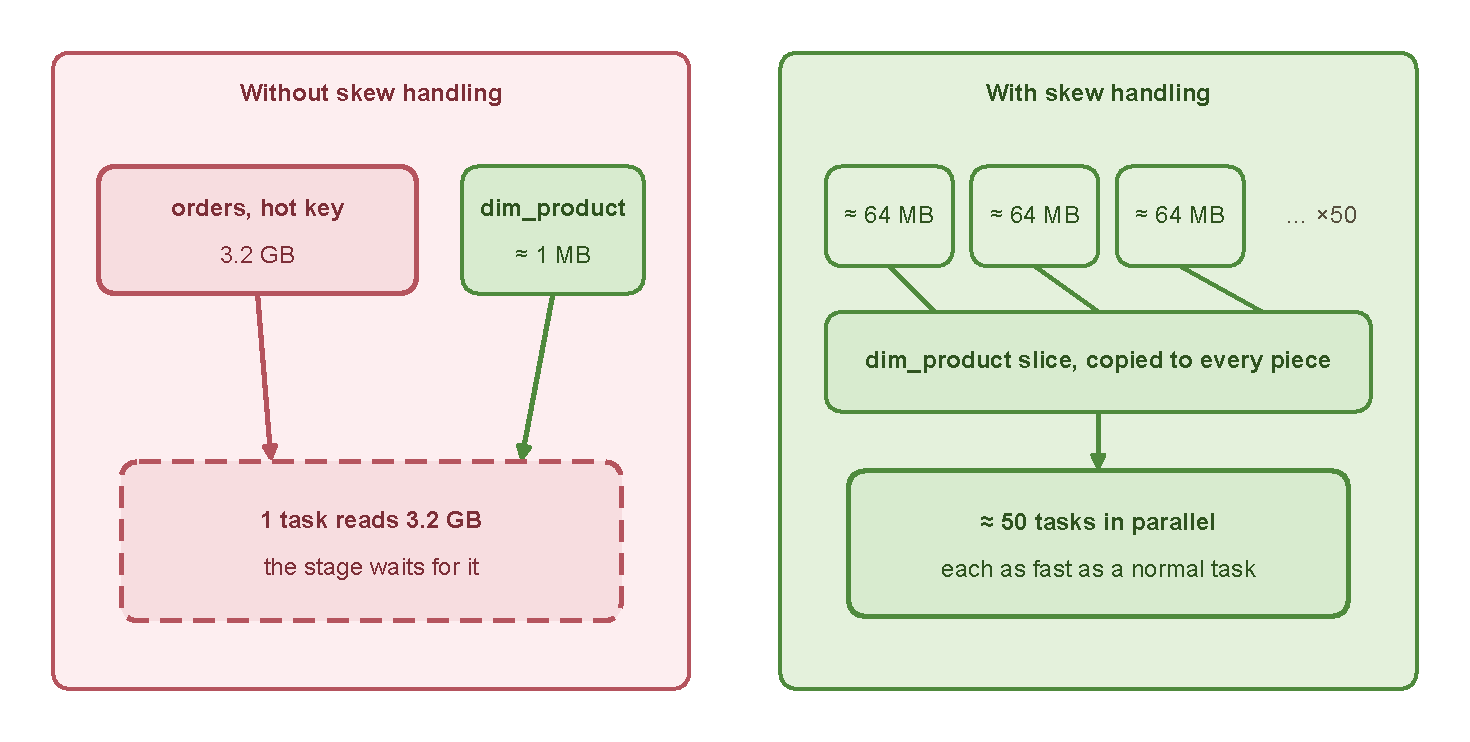
\includegraphics[width=\linewidth]{aqe-skew-split.pdf}
  \caption{Without skew handling, one 3.2~GB partition runs as a single task
  long after the rest of the stage has finished. AQE splits it into pieces near
  the advisory size and copies the small side's slice to each piece, turning one
  straggler into about 50 ordinary tasks.}
  \label{fig:aqe-skew-split}
\end{figure}

The split size is the larger of the advisory size (64~MB) and the average size of
the \emph{non-skewed} partitions. With a 40~MB median, that is 64~MB, so the
3.2~GB partition becomes about $3200 / 64 = 50$ sub-partitions. The split
happens along \emph{map-task boundaries}: each sub-partition is a range of map
outputs for that reducer, so a stage with only 8 map tasks can split a
partition into at most 8 pieces, whatever the target says. (Claim --- verify
against \texttt{createSkewPartitionSpecs} in the 3.5 source and with the capture
below.) On the replicated side, the cost is reading its slice 50 times: for a
1~MB slice of \texttt{dim\_product}, 50~MB of extra reads, which is nothing.

The cost is real when the other side is large. If \emph{both} sides are skewed on
the same key, AQE splits both, and the join runs every pair of pieces: $m \times
n$ tasks over $m + n$ pieces of data. Skew handling is a good trade only because,
in the common case, one side of a skewed join is a small dimension.

Which side can be split depends on the join type, because splitting the wrong
side of an outer join changes the result:

\begin{table}[htbp]
\centering\footnotesize
\renewcommand{\arraystretch}{1.25}
\begin{tabular}{@{}p{4.5cm}p{4.2cm}p{5.0cm}@{}}
\toprule
\textbf{Join type} & \textbf{Left side split?} & \textbf{Right side split?} \\
\midrule
Inner, cross & yes & yes \\
Left outer, left semi, left anti & yes & no \\
Right outer & no & yes \\
Full outer & no & no \\
\bottomrule
\end{tabular}
\caption{Skew handling splits only the side whose rows can be partitioned
without changing the join result. A full outer join cannot be skew-split at all.}
\label{tab:aqe-skew-jointype}
\end{table}

\subsection{Reproducing the straggler}

To study skew on the specimen, remove the escape hatch that would otherwise
broadcast \texttt{dim\_product}, and compare AQE's skew handling on and off:

\begin{lstlisting}[language=SQL,caption={Isolating skew handling on the specimen's join},captionpos=b,label=lst:aqe-skew-experiment]
SET spark.sql.autoBroadcastJoinThreshold = -1;       -- keep the join sort-merge
SET spark.sql.adaptive.skewJoin.enabled = false;     -- run 1: no skew handling
-- run the specimen, then open Stages -> the join stage -> Summary Metrics

SET spark.sql.adaptive.skewJoin.enabled = true;      -- run 2: default behavior
-- run it again and compare max vs median task time
\end{lstlisting}

In the \textbf{Stages} tab, a skewed stage shows it in the Summary Metrics: the
\emph{max} task duration and shuffle-read size sit far above the \emph{median}
(\Cref{sec:shape-ui}). With skew handling on, the same stage should show the max
close to the median, and the join node in the final plan carries
\texttt{isSkew=true}:

\begin{lstlisting}[language=text,numbers=none,caption={The shape of a skew-split join in a final plan},captionpos=b,label=lst:aqe-skew-plan]
AdaptiveSparkPlan isFinalPlan=true
+- ...
   +- SortMergeJoin [product_id], [product_id], Inner, isSkew=true
      :- Sort [product_id ASC NULLS FIRST]
      :  +- AQEShuffleRead skewed
      :     +- ShuffleQueryStage 0
      +- Sort [product_id ASC NULLS FIRST]
         +- AQEShuffleRead skewed
            +- ShuffleQueryStage 1
\end{lstlisting}
% CAPTURE: final plan from lst:aqe-skew-experiment run 2, with the Stages tab Summary Metrics rows (min/25th/median/75th/max) from both runs side by side

If the skew is worse than the defaults catch, lower the two thresholds ---
\conf{skewedPartitionFactor} to 3.0 and \conf{skewedPartitionThresholdInBytes} to
128~MB, say --- at the cost of treating more ordinary variance as skew. Each
false positive spends extra tasks and extra reads of the replicated side. By
default AQE also skips skew handling if applying it would add an extra shuffle
elsewhere in the plan; \conf{spark.sql.adaptive.forceOptimizeSkewedJoin}
(default \texttt{false}, since Spark 3.3) overrides that. (Claim --- verify the
default on 3.5.2.)

\section{Reading an AQE plan}
\label{sec:aqe-reading}

The plan \texttt{EXPLAIN} prints before an action runs is not the plan that ran.
The one that matters is the plan the SQL tab shows after execution, rooted at
\texttt{AdaptiveSparkPlan isFinalPlan=true}. \Cref{lst:aqe-final-plan} is one
final plan, with the decisions AQE made numbered for the walk-through that
follows. It joins \texttt{orders} to the large \texttt{dim\_customer}, so the
join is a real sort-merge join and not one AQE later converts, during the week
of the viral product.

\begin{lstlisting}[language=text,numbers=none,basicstyle=\footnotesize\ttfamily,caption={A final AQE plan, annotated: a skew-split join feeding a coalesced aggregation},captionpos=b,label=lst:aqe-final-plan]
AdaptiveSparkPlan isFinalPlan=true                                   -- (1)
+- *(3) HashAggregate(keys=[segment], functions=[avg(on_time)])
   +- AQEShuffleRead coalesced                                       -- (2)
      +- ShuffleQueryStage 2                                         -- (3)
         +- Exchange hashpartitioning(segment, 2000)
            +- *(2) HashAggregate(keys=[segment], functions=[partial_avg(...)])
               +- *(2) SortMergeJoin [customer_id], [customer_id], Inner, isSkew=true   -- (4)
                  :- AQEShuffleRead skewed                           -- (5)
                  :  +- ShuffleQueryStage 0
                  +- AQEShuffleRead skewed
                     +- ShuffleQueryStage 1
\end{lstlisting}
% CAPTURE: replace with the real final plan; the numbered annotations are authoring aids and stay as comments in the capture

Read it from the root down:

\begin{enumerate}
  \item \textbf{The root.} \texttt{isFinalPlan=true} confirms this is the plan as
        executed. \texttt{isFinalPlan=false} is the compile-time plan from
        \texttt{explain()} before an action; it may differ substantially.
  \item \textbf{Coalescing.} \texttt{AQEShuffleRead coalesced} over the
        aggregation's shuffle: AQE merged its many small partitions before the
        final aggregate ran (\Cref{sec:aqe-coalesce}).
  \item \textbf{Query stage numbers.} The number after \texttt{ShuffleQueryStage}
        identifies one materialization point. The \texttt{Exchange} under it is
        what Catalyst planned, still reading 2000, because coalescing changes the
        read, not the write.
  \item \textbf{The join flag.} \texttt{isSkew=true} on the join marks that skew
        handling applied to \emph{this} join, not just somewhere upstream.
  \item \textbf{Skewed reads.} \texttt{AQEShuffleRead skewed} on a join's inputs
        marks the split side and the replicated side; both inputs of a skew-split
        join carry it.
\end{enumerate}

One query, two unrelated runtime corrections, each visible as its own marker in
the same final plan. A \texttt{BroadcastQueryStage} appears in a different
scenario: in a promoted join, the \texttt{SortMergeJoin} node is gone, replaced
by a \texttt{BroadcastHashJoin} as in \Cref{lst:aqe-broadcast-plan}. A join
cannot show both a skew split and a broadcast promotion on the same side: a
promoted side has no shuffle partitions left to measure for skew. The reference
for every AQE node, including the ones this chapter does not need, is
\Cref{sec:c-aqe}.

\begin{tip}
The \texttt{AQEShuffleRead} node's metrics in the SQL tab report how many
partitions it read, how many it coalesced, and how many it split. Hover the
node to read them: they confirm what the plan's wording only hints at, and they
are the quickest way to check that a rewrite did what you intended.
(Claim --- the exact metric names are worth verifying on your cluster.)
\end{tip}

Where the final plan is not available at all --- a query that has no exchange --- that is
itself information, and the next section says why.

\section{What AQE cannot fix}
\label{sec:aqe-limits}

AQE is the safety net under the decisions the earlier chapters taught, not a
replacement for them. \Cref{tab:aqe-limits} lists the places it does nothing, and
why.

\begin{table}[htbp]
\centering\footnotesize
\renewcommand{\arraystretch}{1.25}
\begin{tabular}{@{}p{4.0cm}p{5.2cm}p{5.0cm}@{}}
\toprule
\textbf{Situation} & \textbf{Why AQE cannot help} & \textbf{What to do instead} \\
\midrule
The first stage: scans and file splits & nothing has run, so there is nothing to measure & size input splits and files (\Cref{sec:shuffle-partition}) \\
A query with no exchange and no subquery & no query stage boundary exists, so AQE does not wrap the plan & nothing to fix; a single-stage plan has no shuffle to re-plan \\
An explicit \texttt{repartition(n)} & the user asked for exactly $n$ partitions, and AQE honors it & use \texttt{repartition} by column, or drop the count \\
Skew in an aggregation, not a join & AQE's skew rule applies to joins only & partial aggregation, or salting the key (\Cref{ch:debugging}) \\
Structured Streaming micro-batches & AQE is not applied to streaming queries in 3.5 (claim --- verify) & size partitions explicitly (\Cref{ch:streaming}) \\
A shuffle planning already committed to & AQE re-plans around the exchange, not through it & bucketing or storage-partitioned joins (\Cref{sec:joins-spj}) \\
Both sides of a join skewed on the same key & splitting both multiplies tasks rather than shrinking them & filter or pre-aggregate the hot key \\
\bottomrule
\end{tabular}
\caption{Where AQE does nothing. Each row names the earlier decision that still
matters.}
\label{tab:aqe-limits}
\end{table}

The pattern in the table is the chapter's closing rule: \textbf{AQE turns a
guess into a measurement, but only for the stages that have not run yet.} That
is why \Cref{ch:shuffle}'s advice to set partitions generously,
\Cref{ch:joins}'s advice to give the planner real statistics, and
\Cref{ch:pruning}'s advice to bucket a repeated join all still stand.

\begin{note}
This chapter is pinned to Spark 3.5.2, and every default quoted comes from the
3.5 documentation. AQE keeps changing between releases --- defaults and rules
have moved across 3.0, 3.2, and 3.3 --- so recheck each key against the
migration guide of the version you actually run before relying on a number here.
\end{note}

\section{Summary}
\label{sec:aqe-summary}

Planning happens before any data moves; AQE runs after every shuffle, when
partition sizes are exact, and re-plans the stages that have not run. The loop
(\Cref{fig:aqe-feedback-loop}) makes three rewrites. It coalesces small
partitions toward a target that is the advisory size, pulled lower by the
cluster's parallelism when the shuffle is small (\Cref{tab:aqe-parallelism-first});
it promotes a sort-merge join to a broadcast when one side's measured shuffle
output clears the adaptive threshold, saving the fetch and the sort but not the
shuffle write (\Cref{tab:aqe-thresholds}); and it splits a partition that is both
far above the median and above an absolute floor, replicating the other side
(\Cref{tab:aqe-skew-example}). Reading the final plan confirms which of these
fired, and \Cref{tab:aqe-levers} turns each symptom into the evidence and the
knob.

\begin{table}[htbp]
\centering\footnotesize
\renewcommand{\arraystretch}{1.25}
\begin{tabular}{@{}p{3.2cm}p{3.9cm}p{3.6cm}p{3.4cm}@{}}
\toprule
\textbf{Symptom} & \textbf{Evidence} & \textbf{Knob} & \textbf{Cost} \\
\midrule
thousands of tiny tasks after a shuffle & no \texttt{AQEShuffleRead coalesced} in the final plan; tiny shuffle-read sizes in \textbf{Stages} & check \conf{coalescePartitions.enabled}; raise the initial partition count & none: coalescing reads existing files \\
too few tasks for the cluster after coalescing & task count below slot count in the stage & keep \texttt{parallelismFirst=true}; lower the advisory size & more, smaller tasks \\
a sort-merge join on a small table & no \texttt{BroadcastQueryStage}; small \texttt{Exchange} data size & raise the adaptive broadcast threshold & driver memory; compressed-bytes caveat \\
one straggler task, max $\gg$ median & \textbf{Stages} Summary Metrics & lower the skew factor and threshold & extra tasks and replicated reads \\
AQE seems to do nothing & no \texttt{isFinalPlan=true} root, or a row of \Cref{tab:aqe-limits} applies & fix the earlier decision & none \\
\bottomrule
\end{tabular}
\caption{The AQE levers: each symptom with the evidence that confirms it, the knob
that moves it, and what the knob costs.}
\label{tab:aqe-levers}
\end{table}

\Cref{ch:pruning} turns from deciding how data moves to deciding how much of it
has to be read at all.

\exercisehead
\begin{exercises}
\item \textbf{Run and observe.} Run \Cref{lst:aqe-skew-experiment} on the
      specimen. Record the max and median task duration of the join stage with
      skew handling off, then on. Report how many tasks the stage ran in each
      case, and find the \texttt{isSkew=true} flag in the second run's final
      plan.
\item \textbf{Read a plan.} In \Cref{lst:aqe-final-plan}, which operators carry
      a runtime decision, and which two nodes would you check first to confirm
      the aggregation's shuffle was coalesced? Rewrite the plan as it would
      look if \texttt{dim\_customer} were small enough to be promoted to a
      broadcast.
\item \textbf{Predict, then check.} A stage's shuffle produces 20 partitions of
      1~MB each on a 16-core cluster. Using the target formula in
      \Cref{sec:aqe-parallelism}, predict how many partitions AQE leaves with
      \texttt{parallelismFirst} on, and with it off. Then run it and compare
      against the \texttt{AQEShuffleRead} metrics.
\end{exercises}
